% 
% Seyyed Ali Mohammadiyeh
% pdflatex.exe -synctex=1 -interaction=nonstopmode -shell-escape "gap-days-2025".tex
% pdflatex -synctex=1 -interaction=nonstopmode -shell-escape "gap-days-2025".tex
% 

\PassOptionsToPackage{colorlinks=true,linkcolor=blue,urlcolor=blue,citecolor=blue}{hyperref}
\documentclass{beamer}

\usepackage{amsmath, amssymb}
\usepackage{xcolor}
\usepackage{listings}

\definecolor{gapgreen}{HTML}{90A959}
\usetheme{default}
\usecolortheme[named=gapgreen]{structure}

\title{LatinSquare Manual}
\author[S. A. Mohammadiyeh]{Seyyed Ali Mohammadiyeh\\
Department of Pure Mathematics, Faculty of Mathematical Sciences\\
University of Kashan, Kashan 87317-53153, I. R. Iran\\
\texttt{alim@kashanu.ac.ir}, \texttt{max@std.kashanu.ac.ir}}
\date{\today}

\lstset{
    basicstyle=\ttfamily\small,
    keywordstyle=\color{gapgreen}\bfseries,
    commentstyle=\color{gray},
    stringstyle=\color{blue},
    showstringspaces=false,
    frame=single,
    breaklines=true
}

\setbeamertemplate{navigation symbols}{}

\setbeamertemplate{footline}{
  \leavevmode%
  \hbox{%
  \begin{beamercolorbox}[wd=.8\paperwidth,ht=2.5ex,dp=1ex,left]{author in head/foot}%
    \hspace{1em}\scriptsize Seyyed Ali Mohammadiyeh -- GAP Days 2025
  \end{beamercolorbox}%
  \begin{beamercolorbox}[wd=.2\paperwidth,ht=2.5ex,dp=1ex,right]{date in head/foot}%
    \scriptsize\insertframenumber{} / \inserttotalframenumber\hspace{1em}
  \end{beamercolorbox}}%
  \vskip0pt%
}

\begin{document}

\begin{frame}
  \titlepage
\end{frame}

% \begin{frame}
%   \frametitle{Table of Contents}
%   \tableofcontents
% \end{frame}

\section{What is a Latin Square?}

\begin{frame}
\frametitle{Definition}
A \textbf{Latin square} of order $n$ is an $n \times n$ array filled with $n$ different symbols, each occurring exactly once in each row and exactly once in each column.
\pause
\begin{itemize}
  \item Often, symbols are the integers $\{1, 2, \dots, n\}$.
  \item No symbol repeats in any row or column.
\end{itemize}
\end{frame}

\begin{frame}
\frametitle{Example of a Latin Square}
Here is a Latin square of order 3:
\[
\begin{bmatrix}
1 & 2 & 3 \\
2 & 3 & 1 \\
3 & 1 & 2 \\
\end{bmatrix}
\]
\pause
Each number appears once per row and once per column.
\end{frame}

% \begin{frame}
% \frametitle{More Examples (Order 4)}
% \[
% \begin{bmatrix}
% 1 & 2 & 3 & 4 \\
% 2 & 3 & 4 & 1 \\
% 3 & 4 & 1 & 2 \\
% 4 & 1 & 2 & 3 \\
% \end{bmatrix}
% \quad
% \begin{bmatrix}
% 1 & 2 & 3 & 4 \\
% 3 & 4 & 1 & 2 \\
% 4 & 1 & 2 & 3 \\
% 2 & 3 & 4 & 1 \\
% \end{bmatrix}
% \]
% \end{frame}

\begin{frame}
\frametitle{Applications}
Latin squares appear in:
\begin{itemize}
  \item \textbf{Statistics:} Experimental design to ensure that treatments are balanced across different conditions, allowing for a more reliable analysis of experimental results.
  \item \textbf{Cryptography:} Encryption algorithms.
  \item \textbf{Game and Puzzle design:} Sudoku is a partial Latin square!
  \item \textbf{Combinatorics:} Designs, finite geometry, etc.
\end{itemize}
\end{frame}

\begin{frame}
\frametitle{Group Theory Relation}
Latin squares are related to group theory and quasigroups.
\end{frame}

\begin{frame}
\frametitle{Historical Notes}
\begin{itemize}
  \item Studied by \textbf{Leonhard Euler} in the 18th century.
  \item Euler's conjecture on orthogonal Latin squares was famous (later disproven for $n=6$).
  \item The Korean mathematician Choi Seok-jeong was the first to publish an example of Latin squares of order nine, in order to construct a magic square in 1700, predating Leonhard Euler by 67 years.
\end{itemize}
\end{frame}

\begin{frame}
\frametitle{Euler's Contribution}
The concept of "Latin square" was inspired by mathematical papers by Leonhard Euler (1707–1783), who used Latin characters as symbols, but any set of symbols can be used: the integer sequence 1, 2, 3 can be replaced by the alphabetic sequence A, B, C.
Euler began the general theory of Latin squares.
\end{frame}

\begin{frame}
\frametitle{Choi Seok-jeong}
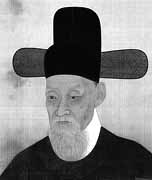
\includegraphics[width=0.5\textwidth]{img12}
Choi Seok-jeong was a Korean politician and mathematician who was the first to find orthogonal Latin squares. He constructed magic squares and invented the Hexagonal Tortoise Problem.
\end{frame}

\begin{frame}
\frametitle{Choi Seok-jeong}
Here is Choi Seok-jeong's orthogonal Latin squares of order 9 in modern notation:
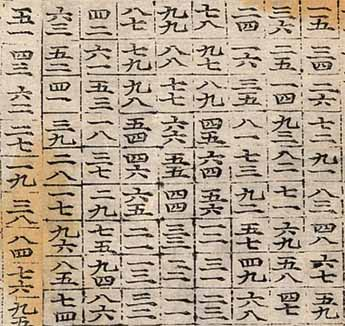
\includegraphics[width=0.5\textwidth]{img10}

From the orthogonal Latin squares, he was able to construct a magic square of order 9.
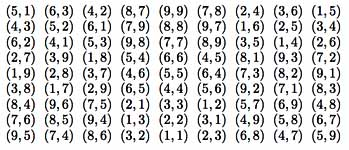
\includegraphics[width=0.5\textwidth]{img11}
\end{frame}

\begin{frame}
\frametitle{Terminology}
\begin{itemize}
  \item \textbf{Order:} The size $n$ of the square.
  \item \textbf{Symbol set:} The $n$ elements used (commonly $1$ to $n$).
  \item \textbf{Orthogonal Latin squares (OLS):} Two Latin squares where each ordered pair occurs once.
  \item \textbf{Mutually orthogonal Latin squares (MOLS):} ...
\end{itemize}
\end{frame}

\begin{frame}
\frametitle{How Many Latin Squares?}
The number grows extremely fast:
\begin{itemize}
  \item $n = 1$: $1$
  \item $n = 2$: $2$
  \item $n = 3$: $12$
  \item $n = 4$: $576$
  \item $n = 5$: $161280$
  \item $n = 6$: over $8.9$ billion!
\end{itemize}
\pause
Exact formulas exist only for small $n$.
\end{frame}

\begin{frame}
\frametitle{Latin Squares in Sudoku}
\begin{itemize}
  \item A valid Sudoku solution is a Latin square with extra region constraints.
  \item Sudoku = Latin square + $3\times3$ box conditions.
\end{itemize}
\begin{center}
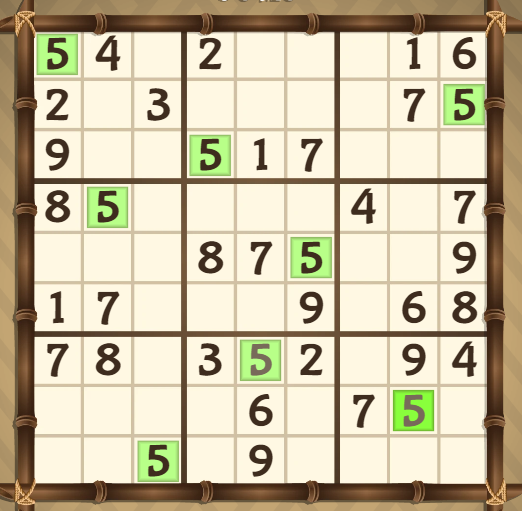
\includegraphics[width=0.5\textwidth]{img8}
\end{center}
\end{frame}

\begin{frame}
\frametitle{Latin Squares in Sudoku}
\begin{center}
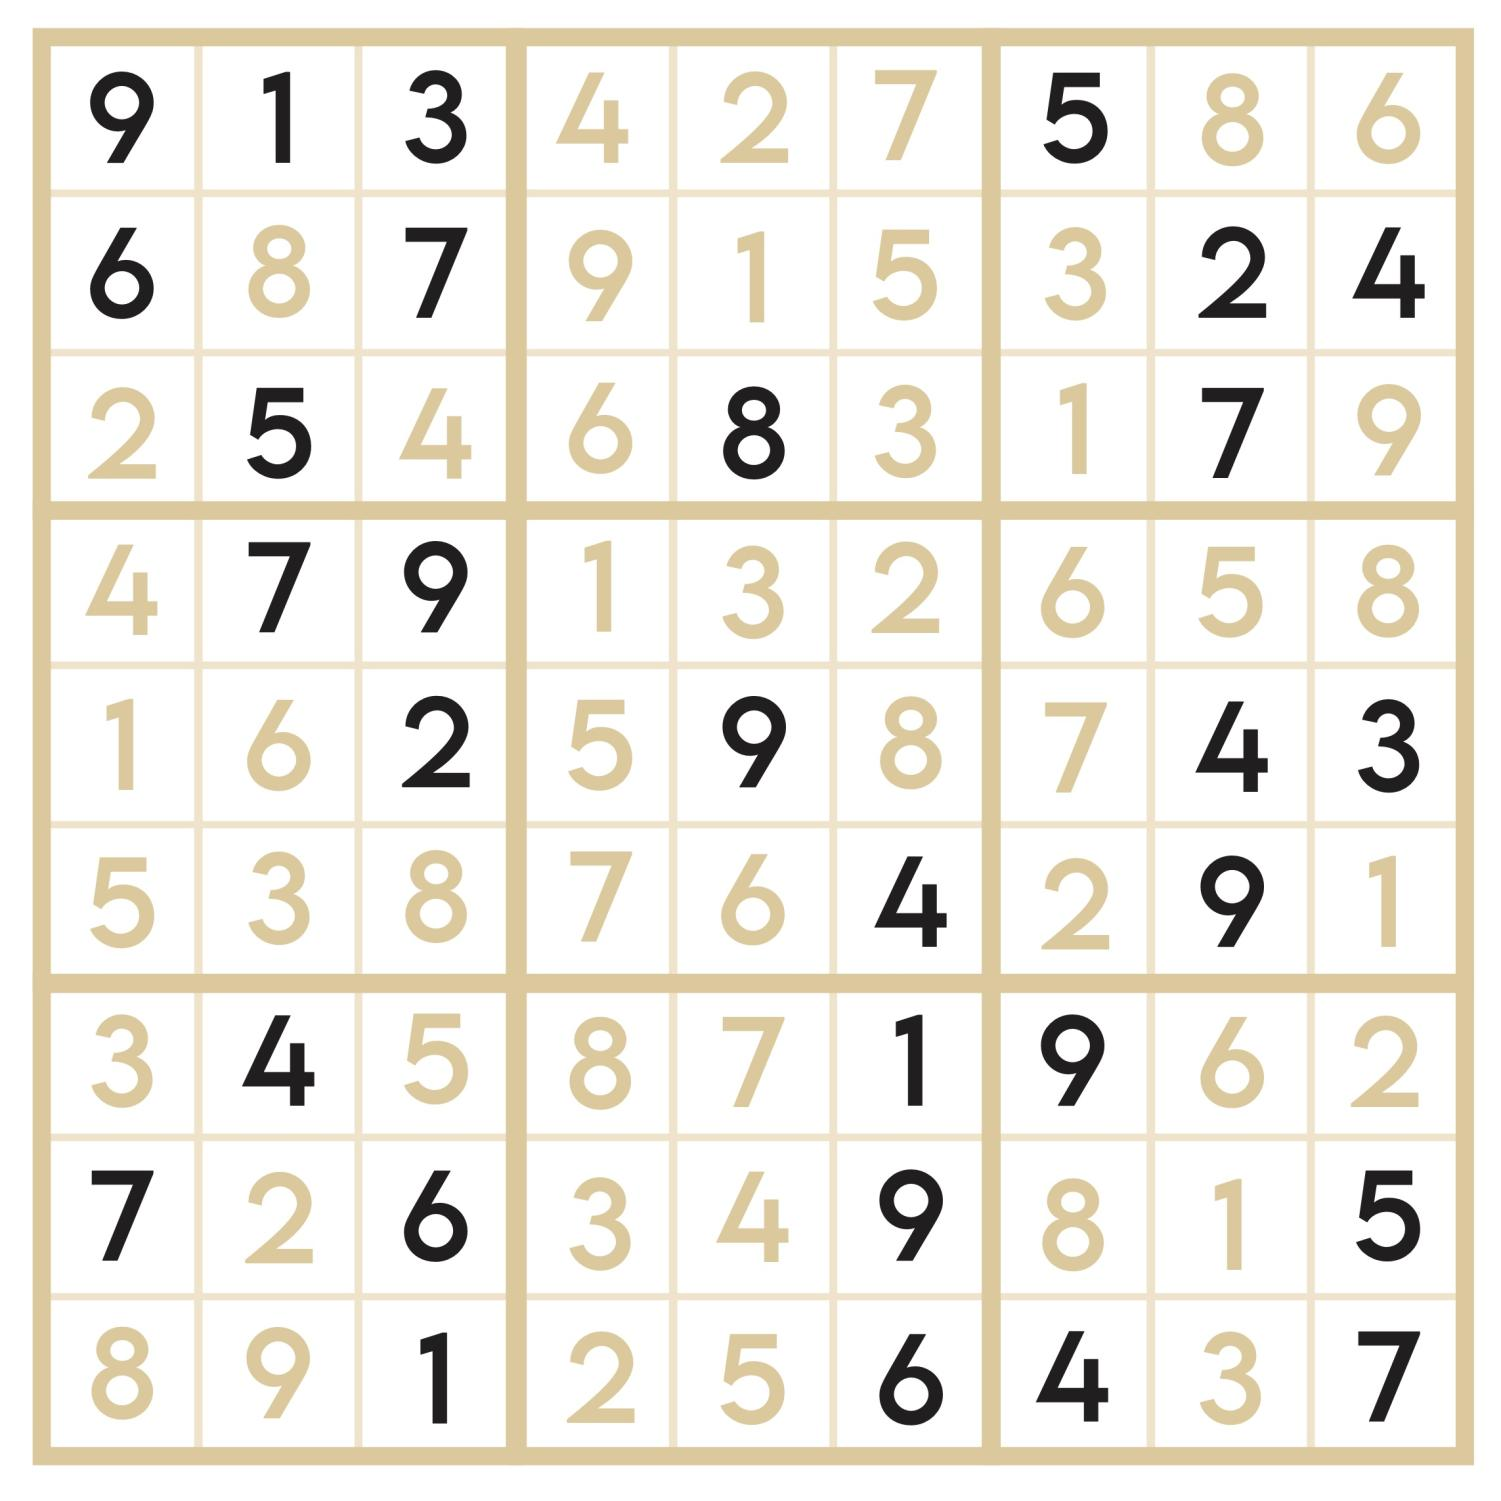
\includegraphics[width=0.5\textwidth]{img9}
\end{center}
\end{frame}

\section{Minimum Order for Latin Squares}
\begin{frame}
\frametitle{Minimum \( n \) for Latin Squares}
\begin{itemize}
  \item A Latin square is a grid filled with \( n \) rows and \( n \) columns, where each number appears exactly once in each row and column.
  \item \textbf{Order 1:} A 1x1 Latin square is trivially possible, as it just contains one element.\\
    Example: \(\begin{bmatrix} 1 \end{bmatrix}\)
  \item \textbf{Order 2:} A 2x2 Latin square is possible. For example:
  \[
  \begin{bmatrix}
  1 & 2 \\
  2 & 1
  \end{bmatrix}
  \]
  \item \textbf{Order 3:} A 3x3 Latin square is the smallest non-trivial Latin square and is possible.
\end{itemize}
\end{frame}

\section{All Latin Squares of Order 1}
\begin{frame}
\frametitle{Latin Squares of Order 1}
The only Latin square of order 1 is:
\[ 
\begin{bmatrix} 
1 
\end{bmatrix} 
\]
\end{frame}

\section{All Latin Squares of Order 2}
\begin{frame}
\frametitle{Latin Squares of Order 2}
There are two Latin squares of order 2:
\[
\begin{bmatrix}
1 & 2 \\
2 & 1
\end{bmatrix}
\quad
\begin{bmatrix}
2 & 1 \\
1 & 2
\end{bmatrix}
\]
These two are isotopically equivalent and represent the cyclic group \( \mathbb{Z}/2\mathbb{Z} \).
\end{frame}

\section{All Latin Squares of Order 3}
\begin{frame}
\frametitle{Latin Squares of Order 3}
There are 12 Latin squares of order 3. One example is:
\[ 
\begin{bmatrix} 
1 & 2 & 3 \\ 
2 & 3 & 1 \\ 
3 & 1 & 2 
\end{bmatrix}
\]
This represents the cyclic group \( \mathbb{Z}/3\mathbb{Z} \).
\end{frame}

\section{All Latin Squares of Order 4}
\begin{frame}
\frametitle{Latin Squares of Order 4}
There are 576 Latin squares of order 4. Here are two examples:
\[
\begin{bmatrix}
1 & 2 & 3 & 4 \\
2 & 3 & 4 & 1 \\
3 & 4 & 1 & 2 \\
4 & 1 & 2 & 3
\end{bmatrix}
\quad
\begin{bmatrix}
1 & 2 & 4 & 3 \\
2 & 3 & 1 & 4 \\
3 & 4 & 2 & 1 \\
4 & 1 & 3 & 2
\end{bmatrix}
\]
\end{frame}

\section{All Latin Squares of Order 5}
\begin{frame}
\frametitle{Latin Squares of Order 5}
There are 161280 Latin squares of order 5. Here are some examples:
\[
\begin{bmatrix}
1 & 2 & 3 & 4 & 5 \\
2 & 3 & 4 & 5 & 1 \\
3 & 4 & 5 & 1 & 2 \\
4 & 5 & 1 & 2 & 3 \\
5 & 1 & 2 & 3 & 4
\end{bmatrix},
\quad
\begin{bmatrix}
1 & 2 & 3 & 5 & 4 \\
2 & 3 & 4 & 1 & 5 \\
3 & 4 & 5 & 2 & 1 \\
4 & 5 & 1 & 3 & 2 \\
5 & 1 & 2 & 4 & 3
\end{bmatrix},
\]
and 161278 more.\\
(You can display these squares across multiple slides if necessary.)
\end{frame}

\begin{frame}
\frametitle{Construction Methods}
Several techniques:
\begin{itemize}
  \item \textbf{Cyclic method:} Rotate rows.
  \item \textbf{Backtracking:} Recursive filling (used in our package).
  \item \textbf{Group-based construction:} Use permutation groups.
\end{itemize}
\end{frame}

\begin{frame}
\frametitle{Recap}
\begin{itemize}
  \item Latin squares are $n \times n$ grids with unique symbols in each row and column.
  \item They have many real-world applications.
  \item Enumeration and generation are key challenges.
\end{itemize}
Next, we'll look at how the GAP package works with Latin squares.
\end{frame}

\begin{frame}
\frametitle{Reduced Latin Squares and Normalized Latin Squares}
Latin squares are also sometimes called "reduced" or "normalized" Latin squares when the first row and first column are in natural order. 
\end{frame}

\begin{frame}
\frametitle{Magic square}
...
\end{frame}

\begin{frame}
\frametitle{Trivial Case}
A 1x1 square is considered trivial because it only contains one cell, and any symbol can be placed there without violating the Latin square property (each symbol appears only once in each row and column).
\end{frame}

\begin{frame}
\frametitle{Non-Trivial}
A Latin square is non-trivial if it has more than one row and column, and each symbol appears exactly once in each row and column.
\end{frame}

\begin{frame}
\frametitle{Smallest Non-Trivial Order}
The smallest order for a non-trivial Latin square is 3, resulting in a 3x3 square.
\end{frame}

\begin{frame}
\frametitle{Balanced Latin Square}
Balanced Latin Squares are special cases of latin square that remove immediate carry-over effects: A condition will precede another exactly once (or twice, if the number of conditions is odd).

The balanced latin square generator proposed and mathematically proved by James V. Bradley in "Complete Counterbalancing of Immediate Sequential Effects in a Latin Square Design".
\end{frame}

\section{latinsquare Package Introduction}
\begin{frame}
\frametitle{Introduction}
This package provides functions to generate and count Latin squares using GAP. It offers:
\begin{itemize}
  \item \textbf{Generation of Latin squares:} Construct all Latin squares of a given order.
  \item \textbf{Counting Latin squares:} Count them without generating all explicitly.
  \item \textbf{Random selection:} Generate all and select one at random.
\end{itemize}
\end{frame}

\section{Functions}
\begin{frame}[fragile]
\frametitle{LatinRow}
\textbf{Prototype:} \texttt{LatinRow(n, r, c)}\\
\textbf{Description:} Computes valid completions of a row for a Latin square of order \texttt{n}.
\begin{lstlisting}
gap> LatinRow(3, [[], [], []], []);
[ [ 1, 2, 3 ], [ 1, 3, 2 ], ... ]
\end{lstlisting}
\end{frame}

\begin{frame}[fragile]
\frametitle{LatinCountRow}
\textbf{Prototype:} \texttt{LatinCountRow(n, k, r, c)}\\
\textbf{Description:} Recursively counts valid completions of the current row.
\begin{itemize}
  \item \texttt{n}: Order of the square.
  \item \texttt{k}: Rows fixed so far.
  \item \texttt{r}: Column restrictions.
  \item \texttt{c}: Current row.
\end{itemize}
\end{frame}

\begin{frame}[fragile]
\frametitle{LatinCount}
\textbf{Prototype:} \texttt{LatinCount(n, k)}\\
\textbf{Description:} Counts all Latin squares of order \texttt{n}, optionally using partial data.
\begin{lstlisting}
gap> LatinCount(3, []);
12
\end{lstlisting}
\end{frame}

\begin{frame}[fragile]
\frametitle{LatinList}
\textbf{Prototype:} \texttt{LatinList(n, c)}\\
\textbf{Description:} Generates all Latin squares of order \texttt{n}.
\begin{lstlisting}
gap> L := LatinList(3, []);
gap> Length(L);
12
\end{lstlisting}
\end{frame}

\section{Usage Examples}
\begin{frame}[fragile]
\frametitle{Counting Latin Squares}
To count the number of Latin squares of order 4:
\begin{lstlisting}
gap> LatinCount(4, []);
\end{lstlisting}
\end{frame}

\begin{frame}[fragile]
\frametitle{Generating Latin Squares}
To generate all Latin squares of order 3:
\begin{lstlisting}
gap> L := LatinList(3, []);
gap> Print(L, "\n");
\end{lstlisting}
\end{frame}

\begin{frame}[fragile]
\frametitle{Random Latin Square}
To randomly select one:
\begin{lstlisting}
gap> L := LatinList(3, []);
gap> RandomLatin := L[ Random(Length(L)) ];
gap> Print(RandomLatin, "\n");
\end{lstlisting}
\end{frame}

\section{Algorithm Overview}
\begin{frame}
\frametitle{Algorithm Overview}

Backtracking, a problem-solving technique in computer science, is generally considered a good and powerful approach for exploring multiple possibilities systematically and finding solutions, especially when dealing with constraints and complex problems. 

This package uses recursive backtracking:
\begin{itemize}
  \item \texttt{LatinRow}: Valid row generation.
  \item \texttt{LatinCountRow}: Counts completions via recursion.
  \item \texttt{LatinList}: Builds full Latin squares.
\end{itemize}
\end{frame}

\section{Installation}
\begin{frame}[fragile]
\frametitle{Installation and Loading}
\textbf{Installation:}  
Place the package inside GAP's \texttt{pkg} directory.\\
\textbf{Loading:}
\begin{lstlisting}
gap> LoadPackage("LatinSquareGAP");
\end{lstlisting}
You should see a confirmation message.
\end{frame}

%\section{License and Author}
%\begin{frame}
%\frametitle{License and Author}
%\textbf{License:} MIT License\\[1mm]
%\textbf{Author:} Seyyed Ali Mohammadiyeh
%\end{frame}

\section{Q\&A}
\begin{frame}
	\frametitle{Thank You!}
	\centering
	\Large Thank you so much for your attention!\\[1em]
	\Large Any questions?
\end{frame}

\section{Acknowledgements}
\begin{frame}
\frametitle{Acknowledgements}
Thanks to the GAP community and contributors who supported this work!
\end{frame}

\begin{frame}[allowframebreaks]
\frametitle{References}
\begin{thebibliography}{99}
\bibitem{gap} GAP Group. GAP -- Groups, Algorithms, Programming, Version 4.11.1; 2023. \url{https://www.gap-system.org}
\bibitem {r1} Ackoff, R. L. (1953). The design of social research. Chicago: University of Chicago Press.
\bibitem {r2} Edwards, A. L. (1998). Experimental design. N.Y.: Addison-Wesley.
\bibitem {r3} Keppel, G. (2006). Introduction to design and analysis. New York: NY: Worth.
\bibitem {r4} Mason, R. L., Gunst, R. F., \& Hess, J. C. (1989). Statistical design and analysis of experiments. New York: NY: Wiley.
\bibitem {r5} Myers, J. L,. & Well, A. D. (2003). Research design and statistical analysis. Mahwah, NJ: Erlbaum .
\bibitem {r6} St Andrews University. (n.d.). Choi Seok-jeong. Retrieved from \url{https://mathshistory.st-andrews.ac.uk/Biographies/Choi_Seok-jeong/}
\end{thebibliography}
\end{frame}

\end{document}
